\subsubsection{Purpose}
The user who wants to subscribe to the \emph{PowerEnJoy} service can carry out the registration process through the mobile application or the web one. First of all the user has to fill a registration form with his/her personal information and accept the Terms and Conditions of use otherwise the procedure will be aborted.

As soon as the user submits the data, the system checks all the information and sends a confirmation e-mail to the specified e-mail address including the password to access the service and the personal PIN required to start the car engine.

\subsubsection{Scenario 1}
Marta would like to register to the \emph{PowerEnJoy} rental service from her computer. She opens the browser and loads the registration page by clicking on the "sign up" button located in the \emph{PowerEnJoy} login page. She fills in the registration form and agrees the service Terms and Conditions. Then Marta submits everything to the system, that checks the personal data. Personal PIN and password are sent to Marta in a confirmation e-mail notifying the successful registration.

\subsubsection{Scenario 2}
Yuri cannot afford a car and therefore decides to take advantage of the \emph{PowerEnJoy} service. He accesses the login page from his mobile phone and taps the "sign up" button since he is not a registered user. Then he fills in the form and accepts the Terms and Conditions of use.

Unfortunately he forgets to fill in his own tax code and the system does not allow him to carry out a successful registration notifying the forgetfulness. Afterwards Yuri completes the procedure by filling the whole form. The system communicates the successful registration and sends him a confirmation e-mail containing PIN and password.

\subsubsection{Use-case}

The use-case of the registration procedure is analyzed in Table \ref{register_uc}.

\subsubsection{Activity diagram}

The activity diagram of the registration procedure is shown in Figure \ref{register_act}.

\subsubsection{Functional requirements}
\begin{enumerate}
\item The user must not enter an already registered e-mail address to perform the registration process;
\item The user must provide the following personal information:
	\begin{itemize}
	\item e-mail address
	\item name
	\item surname
	\item ID card number
	\item tax code
	\item license ID number
	\item address
	\item phone number
	\item credit/prepaid card or \emph{PayPal\textsuperscript{TM}} account credentials
	\end{itemize}
\item There must not be another subscribed user with the same identity card number, tax code or license ID;
\item If the user does not agree the Terms and Conditions of use, the registration process is canceled;
\item The system must send an e-mail containing PIN and password to the e-mail address specified by the user when he/she clicks on "Submit" button and all the required information has been entered;
\item The system allows the user to exit the registration process at any time;
\item The system must allow the user to provide either a valid credit/prepaid card number or \emph{PayPal\textsuperscript{TM}} account credentials to perform the payments;
\item The PIN provided by the system in the confirmation e-mail is made by only digits and has a length of 6;
\item The password provided by the system in the confirmation e-mail is made by both digits and letters (capital and not) and has a length of 8.
\end{enumerate}

\begin{table}[H]
\begin{center}
\begin{tabular}{p{0.3\textwidth} | p{0.7\textwidth}}
\hline
Actor & User\\
\hline
Goal & Goal 1\\
\hline
Input Condition & The user wants to subscribe to the service.\\
\hline
Event Flow & 
\begin{enumerate}
\item The user opens the \emph{PowerEnJoy} home page or the mobile application and clicks or taps on the "Sign up" button;
\item The registration form is loaded and the user fills in all the fields with his/her personal information;
\item The user agrees the service Terms and Conditions by checking the corresponding box;
\item The user clicks on "Submit" button;
\item The system saves the data in its database and sends a confirmation e-mail containing PIN and password to the new registered user.
\end{enumerate} \\
\hline
Output Condition & The system tells the user he/she is successfully subscribed and lets him/her to log in with the provided credentials.\\
\hline
Exception & When some exceptions occur, the system reloads the registration form and goes back to step 2 of Event Flow notifying the user about the error. This happens when the following requirements are not satisfied: 1, 2, 3.

The registration process is aborted when the user decides not to carry it out completely or when requirement 4 generate an exception.\\
\hline
\end{tabular}
\end{center}
\caption{Register use-case}
\label{register_uc}
\end{table}

\begin{figure}[H]
\begin{center}
		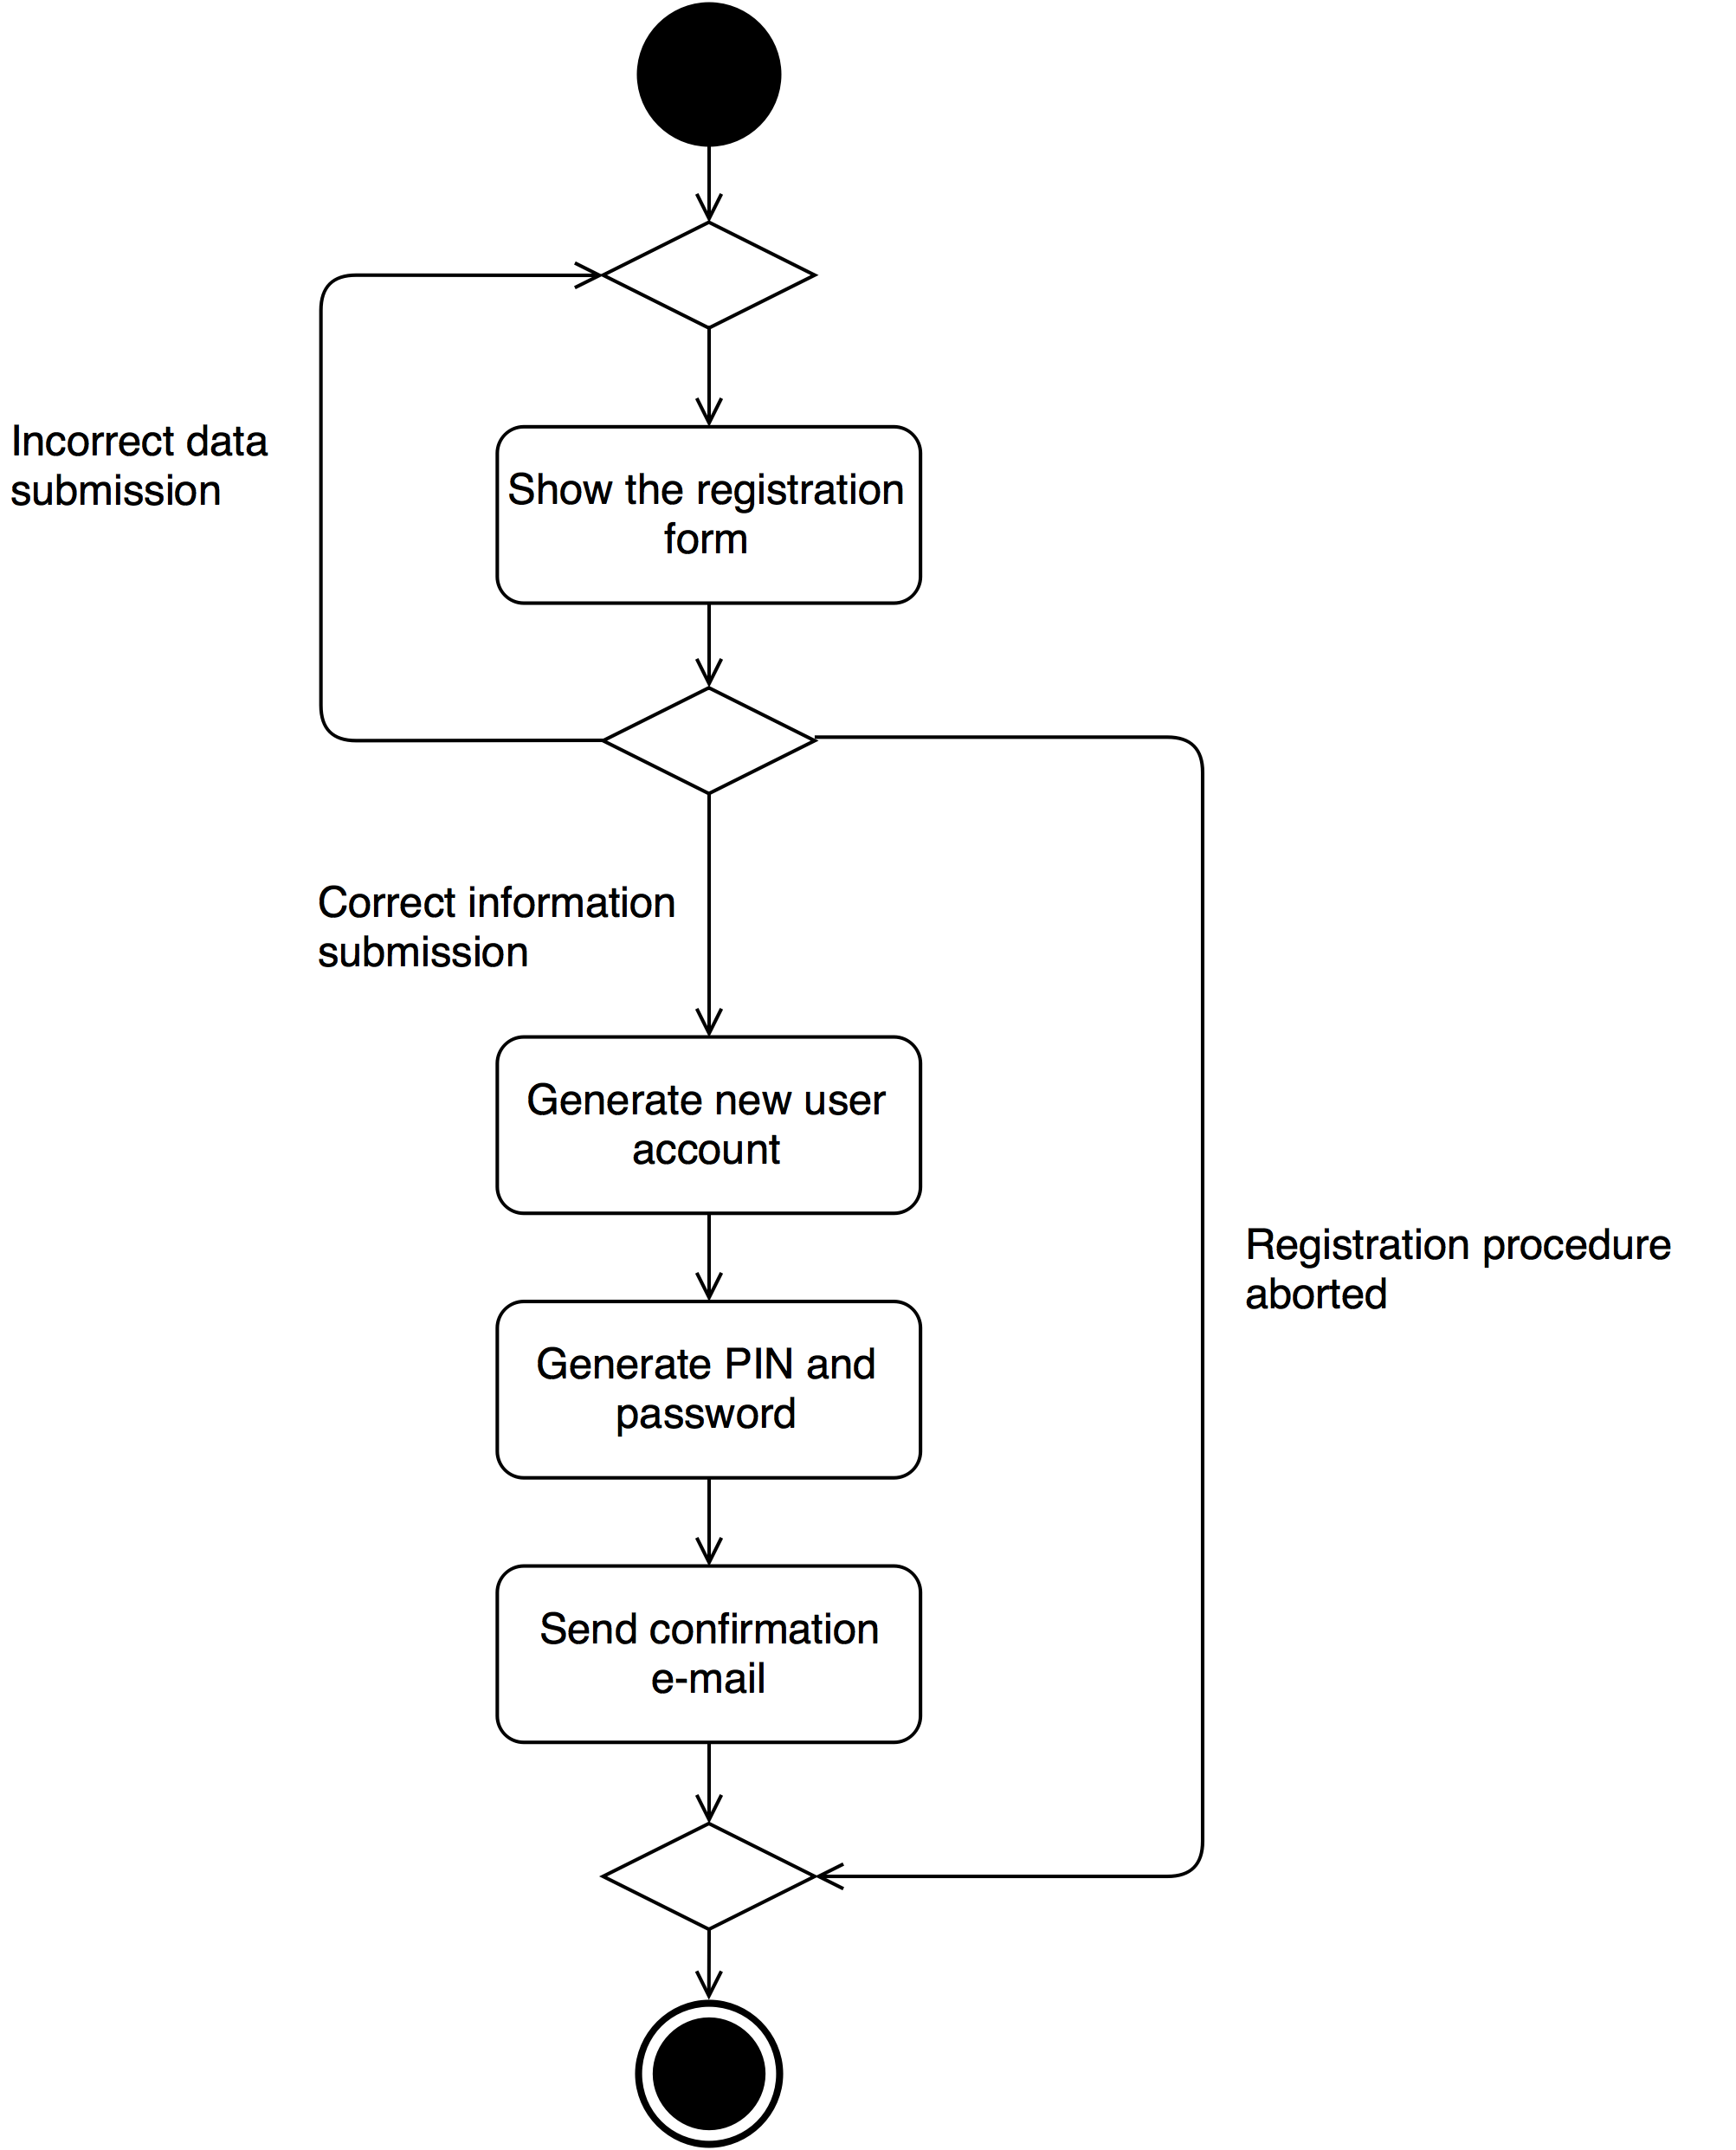
\includegraphics[width=\textwidth]{./specific_requirements/features/diagrams/registration_activity.png}
		\caption{Activity diagram of the registration process from the system point of view}
		\label{register_act}
\end{center}
\end{figure}

\begin{figure}[H]
\begin{center}
		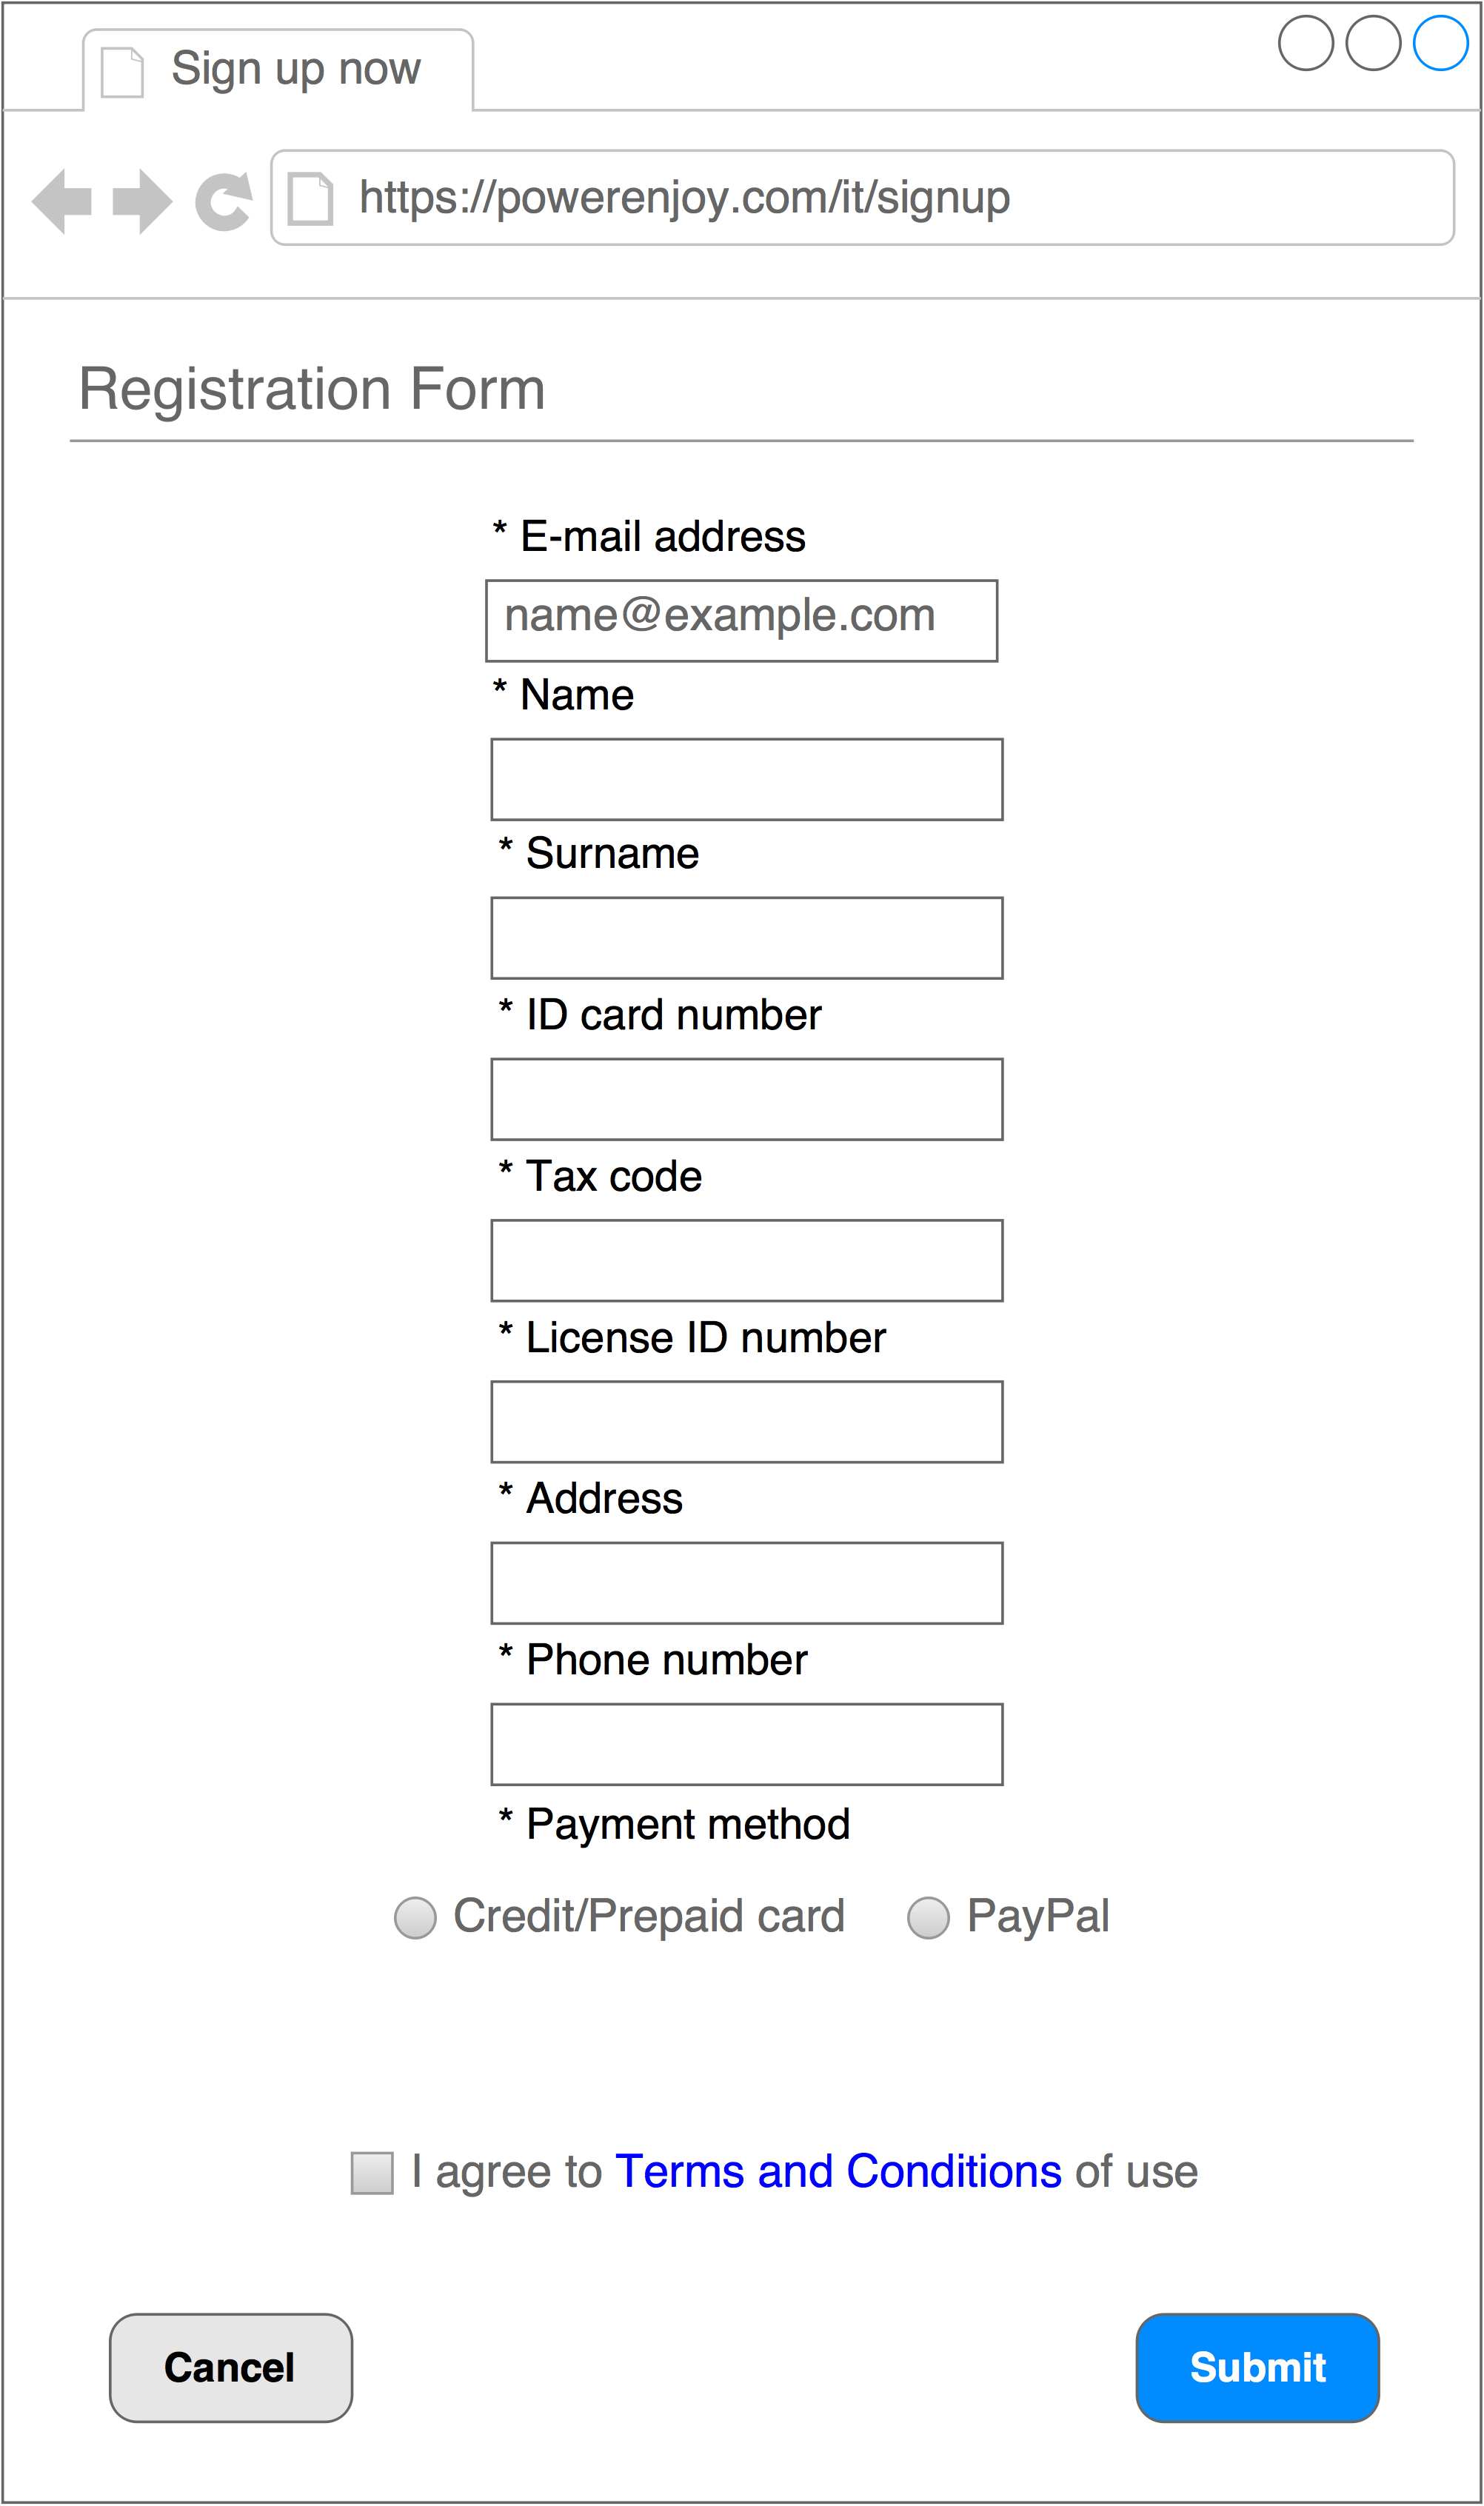
\includegraphics[width=0.8\textwidth]{./specific_requirements/features/diagrams/web_registration.png}
		\caption{Concept of the sign up webpage}
\end{center}
\end{figure}